
\section{Übersicht}
\subsection{DNA Sequenzierungen - Generelle Voraussetzungen}

Alle Sequenzierungsmethoden unterliegen folgenden 3 Voraussetzungen: 

\begin{enumerate}
    \item Die \gls{Leseweite} ist begrenzt. Somit kann es nicht auf beliebiger Länge angewandt werden.
    \item Die DNA muss in ausreichender Reinheit und Konzentration vorliegen.
    \item meist eine Art von Anreicherung identischer DNA-Moleküle notwendig.
\end{enumerate}

\subsection{Einordnung}
\begin{table}[H]
    \centering
    \begin{tabular}{p{4cm}|p{5cm}|p{5cm}}
        \textbf{Klassische Methoden} & \textbf{Next Generation} & \textbf{3rd Generation}  \\ && \\
        Maxam-Gilbert &  Pyrosequencing & Pacific Biosciences SMRT Sequencing \\ && \\
        Sanger &  Illumina Sequencing by Synthesis (SBS) & Oxford Nanopore Sequencing \\ && \\
        & Ion Torrent Semiconductor Sequencing &
    \end{tabular}
    \caption{Arten von Sequenzierungsmethoden nach Generation.}
    \label{tab:seq-gen}
\end{table}

\begin{mybox}[title=Wie unterscheiden sich die Generationen?]
TODO
\end{mybox}

\section{1st Genereation Sequenzierungen}
\index{Sequenzierung!1st Genereation}

\subsection{Die Maxam-Gilbert-Methode (Chemische Spaltung)}\index{Maxam-Gilbert-Methode}
Die Methode braucht einsträngige DNA Fragmente, die an den 5'-Enden radioaktiv markiert sind.\\ 
Die Methode funktioniert über Chemische Spaltung an Nukleotiden.
Hierzu werden immer vier Proben mit den folgenden vier Spaltungen angefertigt:
\begin{itemize}
    \item G
    \item G + A 
    \item T + C
    \item C
\end{itemize}
D.h. es werden vier "verschiedene Versuche" durchgeführt, in einem wird immer an G gespalten, in der anderen an G und A usw. Die Produkte werden dann durch Elektrophorese größengetrennt und man man kann anhand der verschiedenen Banden ablesen, welche Base vorliegt. Ein Band entspricht einer der Spaltungsproben. 
\begin{figure}[H]
    \centering
    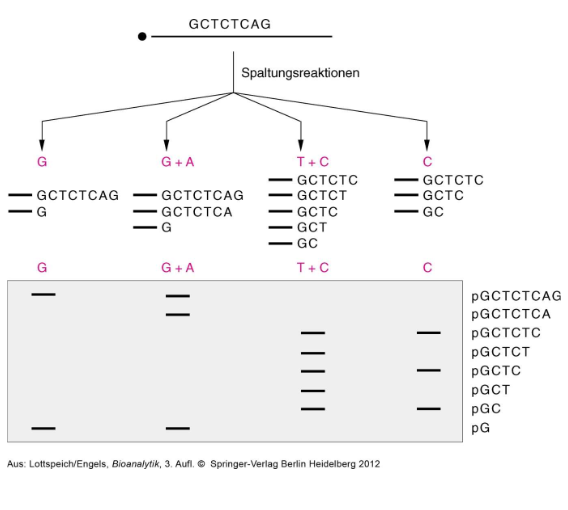
\includegraphics[width=0.8\linewidth]{images/Maxam-Gilbert.PNG}
    \caption{Maxam-Gilbert Elektrophorese}
    \label{fig:enter-label}
\end{figure}
\noindent Für ein G muss bei der Bande für G, als auch bei der Bande G + A eine Bande erkennbar sein.\\
Für A nur bei G + A. \\
Für T bei T + C. \\
Für C bei T + C und C.

\subsection{Sanger-Sequenzierung (Didesoxymethode)}
\subsubsection{Ablauf}
\begin{enumerate}
    \item Der Primer bindet an das 5'-Ende eines komplementären Stranges (Matrize/Template-DNA) und wird vom 3'-OH-Ende aus mit einer DNA Polymerase verlängert.
    \item Einbau von Nukleotiden: 
    \begin{itemize} 
        \item Desoxynukleotide (\glspl{dntp}: dATP, dCTP, dGTP, dTTP)
        \item Didesoxynukleotide (\glspl{ddntp}: ddATP, ddCTP, ddGTP, ddTTP)
    \end{itemize}
    \item Einbau von \gls{ddntp} führt zum Syntheseabbruch, da solches keine OH Gruppe am 3' Ende besitzt können keine weiteren Nukleotide angehängt werden. 
\end{enumerate}
Daraus resultieren verschieden lange Abschnitte, die aus der Template-DNA "kopiert" wurden und immer an der gleichen Stelle beginnen (wo der Primer war) und immer in einem markierbaren Nukleotid enden. Wann ein \gls{ddntp} eingebaut wird, ist Zufall.  \\ Die \glspl{ddntp} können durch radioaktive Isotope (früher) und Fluoreszenzfarbstoffe (heute) markiert werden. \newline
Wenn man diese Stücke nun durch Gelelektrophorese ihrer Größe nach aufteilt und die Markierungen ausliest, kann man die Sequenz rekonstruieren (siehe Abb. \ref{fig:sanger}).
\begin{figure}[H]
    \centering
    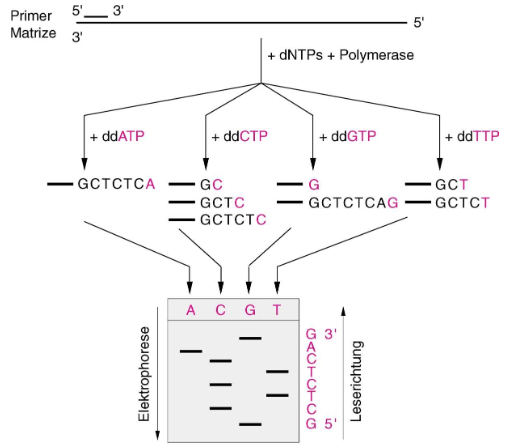
\includegraphics[width=0.8\linewidth]{images/Sanger.PNG}
    \caption{Ablauf der Sanger Sequenzierung. Bei der Abbildung ist zu beachten, dass vier verschiedene Absätze (einer für jede Base) erstellt werden und nicht alle \glspl{ddntp} zusammen gemischt werden.}
    \label{fig:sanger}
\end{figure} \index{Sequenzierung!Sanger}
\noindent Nachteil ist, dass die Interpretation der Ergebnisse
\begin{itemize}
    \item Expertenwissen erfordert.
    \item langsam und arbeitsintensiv ist.
    \item NICHT automatisiert werden kann.
\end{itemize}       
\begin{mechanism}[title=Wie ist der Ablauf von Sanger Sequencing?]
\begin{enumerate}
    \item 1. Primer bindet and 5’ ende des komplementären Stranges und wird mit
einer DNA Polymerase verlängert.
\item 2. Es werden dann Desoxynukleotide (dNTP) bis zur vorletzten Position
angehängt.
dNTP’s sind: dATP, dCTP, dGTP, dTTP
\item 3. Das letzte Nukleotid ist ein Didesoxnukleotid (ddNTP). Da solches keine
OH Gruppe am 3’ Ende besitzt können keine weiteren Nukleotide ange-
hangen werden. Somit ist dann die Sequenzierung zuende!
ddNTP’s sind: ddATP, ddCTP, ddGTP, ddTTP
\end{enumerate}
\end{mechanism}
\begin{mechanism}[title=Prinzip der Sanger Sequenzierung und seiner Nachweis- u. Detektionsmethoden?]
Kettenabbruchmethode: Während der DNA-Synthese durch die DNA-Polymerase werden die ddNTPs zufällig in die wachsende DNA-Kette eingebaut. Wenn ein ddNTP eingebaut wird, stoppt die Verlängerung der DNA-Kette, da keine weitere Bindung möglich ist. \\ Dieser Prozess führt zu einer Mischung von DNA-Fragmenten unterschiedlicher Länge, die jeweils mit einem ddNTP enden. Jedes ddNTP ist typischerweise mit einem einzigartigen Fluoreszenzfarbstoff markiert.
\end{mechanism}\index{Sequenzierung!Sanger}
\begin{mechanism}[title=Wichtige Komponenten und Enzyme der Sanger-Sequenzierung]
\begin{itemize}
    \item \glspl{dntp}
    \item \glspl{ddntp}
    \item DNA-\gls{Polymerase}
    \item Pufferlösung
    \item Fluoreszenzfarbstoffe
\end{itemize}
\end{mechanism}

\subsubsection{Weiterentwicklung}

\paragraph{Nicht radioaktive Marker} zu verwenden ist eine der Weiterentwicklungen der Sanger-Sequenzierung. Heute werden Fluoreszenz-Farbstoffe benutzt, was das automatisierte Lesen von Sequenz-Daten erlaubt. Und durch die Verwendung von verschiedenen Farbstoffen kann man alle Nukleotide in einem Ansatz vermischen und braucht nicht einen Ansatz pro Base.  

\begin{figure}[H]
    \centering
    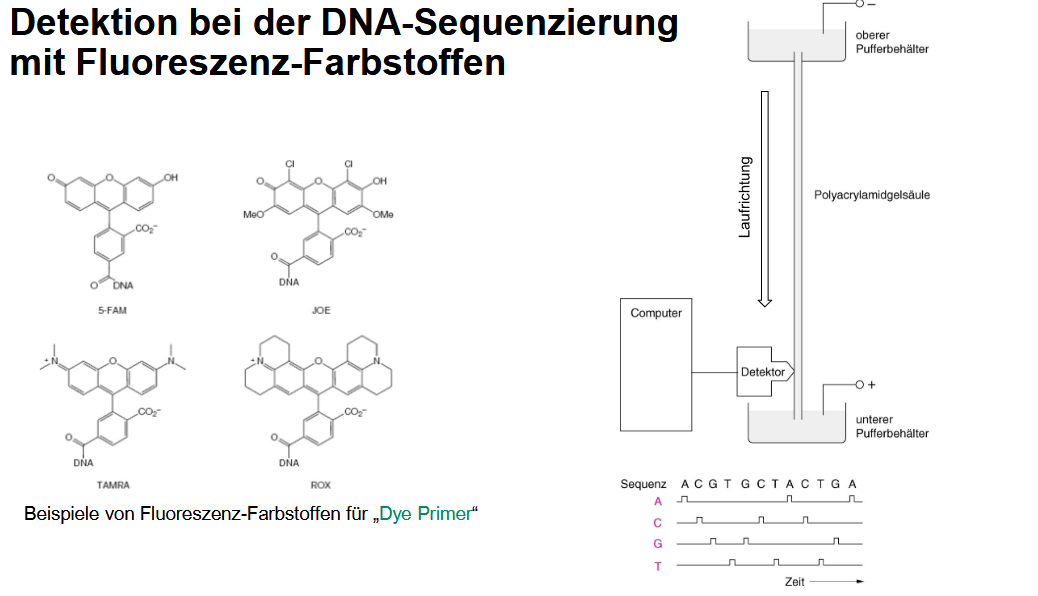
\includegraphics[width=0.7\linewidth]{images/Floreszenz Farbstoffe.PNG}
    \caption{Unterschiedliche nicht radioaktive Fluoreszenzen, mit denen \glspl{ddntp} markiert werden können.}
    \label{fig:enter-label}
\end{figure}
\begin{figure}[H]
    \centering
    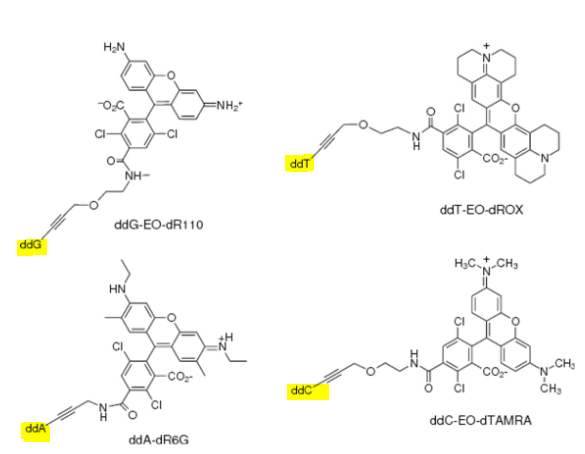
\includegraphics[width=0.6\linewidth]{images/ddNTP Marker.PNG}
    \caption{ddNTP mit Markern}
    \label{fig:enter-label}
\end{figure}
\noindent \textbf{Ablauf des Einlesens:} Die markierte Proben werden mit einem Laser angeregt und Licht wird durch einzelne Banden emittiert und als Pixel-Grafik aufgezeichnet.
Die Daten können mit spezieller Software gelesen werden (automatisierte Basecaller).\index{automatisiertes Basecalling}

\paragraph{"Cycle Sequencing"}\index{Cycle Sequencing} ist eine Verbesserung der Sanger-Sequenzierung durch den Einsatz thermostabiler DNA-Polymerasen aus PCR. Dies erlaubt eine mehrfache zyklische Wiederholung der Sequenzierreaktion unter „Wiederverwendung“ der Template-DNA.  \\
Außerdem gibt es eine geringere Anforderungen an Template-DNA-Konzentration, da automatisierte Plasmid-DNA Isolation möglich ist. \\
Die erhöhte Signalintensität (durch mehrere Zyklen) führt zu höheren Leseweiten. 
\begin{mybox}[title=Wie unterscheiden sich PCR und Cycle Sequencing?]
Bei der PCR werden zwei Primer verwendet und beim CS nur einer. Außerdem steigt bei der PCR die Produktkonzentration mit der Anzahl der Zyklen exponentiell an und beim CS nur linear. 
\end{mybox}

\paragraph{Automatisierung durch Kapillar Elektrophorese} \index{Kapillar Elektrophorese}
\begin{figure}[H]
    \centering
    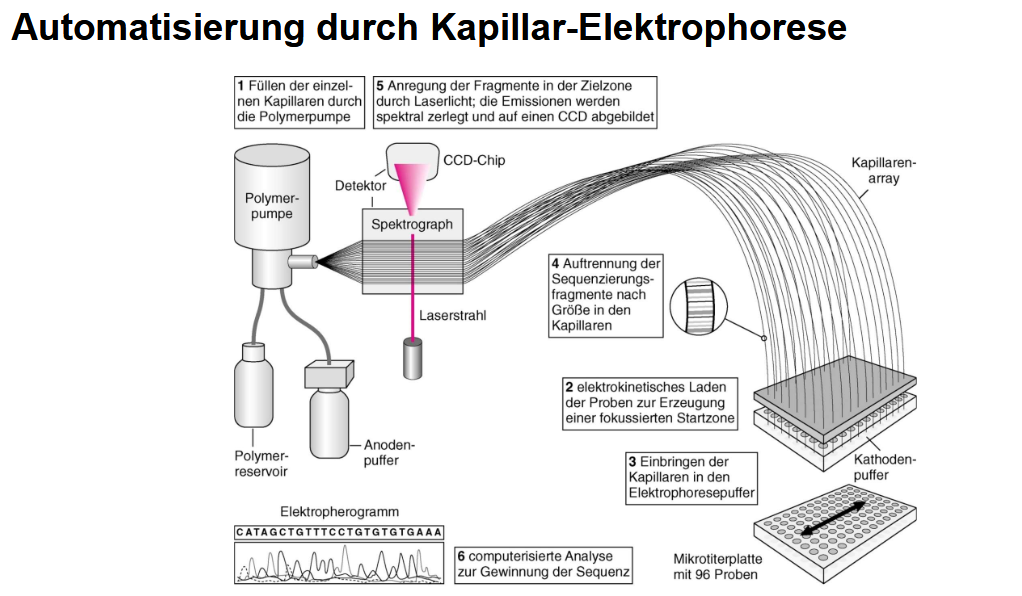
\includegraphics[width=1.0\linewidth]{images/Kapillar elektrophorese.PNG}
    \caption{Ablauf der Kapillar Elektrophorese}
    \label{fig:enter-label}
\end{figure}


\section{2nd Generation Sequenzierung} \index{Sequenzierung!2nd Generation}
\subsection{454 Sequenzierung (Pyrosequenzierung)} \index{Sequenzierung!Pyro}
\begin{enumerate}
    \item Bibliothek-Herstellung
    \begin{itemize}
        \item Die DNA wird fraktioniert 
        \item Polishing der Strang-Enden zu glatten Enden
        \item  Das 5' Ende bekommt einen Adapter B, was ein Biotin-Tag zur Anheftung von \gls{streptavidin}-Mikrokügelchen ist
        \item  Das 3' Ende bekommt Adapter A was für die Amplifikation und Sequenzierung gedacht ist
        \item Herstellung von \gls{sstdna} Einzelsträngen (mit Adaptern)
        \item Titration
    \end{itemize}
    \item \gls{empcr}
    \begin{itemize}
        \item Die \gls{sstdna} wird dann über Adapter B an Mikrokügelchen gekoppelt und in Wasser-Öl Emulsion amplifiziert und kloniert
    \end{itemize}
    \item Vorbereitung der Sequenzierung
    \begin{itemize}
        \item Die Mikrokügelchen werden in eine Picotiterplatte verteilt (jeweis ein Beats in einen "Well". ein Well ist ein warbenförmiges Loch)
        \item Enzyme zur Abdeckung der wells werden hinzugegeben
        \item Zentrifugation
    \end{itemize}
    \item Pyrosequenzierung \index{Sequenzierung!Pyro}
    \begin{enumerate}
        \item Nukleotide werden schrittweise zugegeben.
        \item Wenn eine DNA-Polymerase ein Nukleotid einbaut, wird Pyrophosphat (PPi) freigesetzt.
        \item PPi wird von Enzymen (ATP-Sulfurylase, Luciferase) in Lichtsignale umgewandelt.
        \item Eine Kamera erfasst diese Lichtsignale und bestimmt die DNA-Sequenz. \\
        \begin{figure}[H]
            \centering
            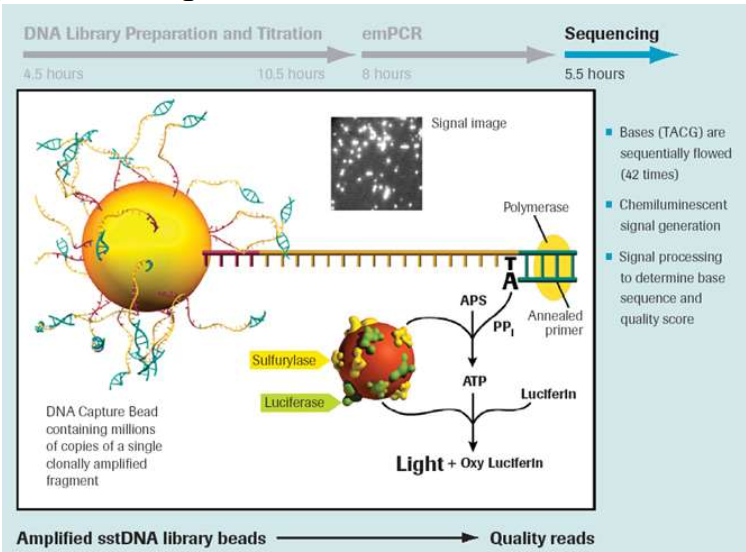
\includegraphics[width=0.8\linewidth]{images/Pyrosequenzierung.PNG}
            \caption{Bild der Pyrosequenzierung mit Sulfurylase und Luciferase}
            \label{fig:enter-label}
        \end{figure}
    \end{enumerate}
\end{enumerate}
\begin{mechanism}[title=Welcher Schritt ist ausschlaggebend für die Pyrosequenzierung? In welchem Schritt wird detektiert?]
Wenn die DNA-Polymerase ein Nukleotid einbaut, so wird Pyrophosphat (PPi) freigesetzt.\\
Solches ist entscheident, da es durch die Enzyme ATP-Sulfurylase und Luciferase in Lichtsignale umgewandelt wird. \\
Das Detektieren passiert ganz am Ende, indem eine Kamera die Lichtsignale aufzeichnet.
\end{mechanism}\index{Sequenzierung!Pyro}


\subsection{Illumina Sequenzierung}\index{Sequenzierung!Illumina}
Detaillierter Ablauf:
\begin{enumerate}
    \item \textbf{Library preparation (Whole Genome Shotgun)}
    \begin{itemize}
        \item Material: gereinigte genomische DNA
    \end{itemize}
    \begin{enumerate}
        \item Fragmentierung der DNA
        \item Reparatur der Enden (Stumpfe 5'-Enden)
        \item Erstellung der 3‘dA Überhänge
        \item Anhängen der Adapter
        \item Entfernen aller freien Adapter, die sich nicht ligiert haben
        \item Kapillare Gelelektrophorese zur Auswahl der Fragmentlängen 
    \end{enumerate}
    \item \textbf{Erstellung der Cluster} durch Bridge Amplification auf einer Flow Cell 
     \begin{itemize}
        \item Material: Flowcell auf deren Oberfläche zu den Adaptern komplementäre Oligonukleotide befestigt sind
    \end{itemize}
    \begin{enumerate}
      \item die Fragmente der Library werden mit den Oligonukleotiden hybridisiert
        \item Es werden mit den gebundenen Strängen als Template an den Oligonukleotiden der Flow Cell Doppelstränge synthetisiert 
        \item Denaturierung und die ursprünglichen DNA Stränge werden verworfen, es bleiben nur die an den Oligonukleotiden hybridisierten 
        \item Die gebundenen DNA-Fragmente beugen sich und ligieren sich mit ihrem zweiten Adapter ebenfalls an gebundene Oligonukleotiden und formen dabei Brücken
        \item Eine DNA-Polymerase synthetisiert aus dem zweiten nun verbundenen Oligonukleotid ebenfalls einen ganzen Strang -> dsDNA-Brücke
        \item Denaturierung und Wiederholung
        \item Der Gegenstrang wird abgeschnitten und verworfen 
        \item Frei 3'-Enden werden blockiert
    \end{enumerate}
    \item \textbf{Sequencing-by-Synthesis}
    \begin{enumerate}
     \item Sequenzierungsprimer werden an Adaptersequenzen hybridisiert 
        \item Der Primer wird Base für Base verlängert mit fluoreszent markierten und vor weiterer Verlängerung geschützten Basen 
        \item Der Fluoreszentpartikel wird per Laser angeregt und das Signal ausgelesen 
        \item die Schutzgruppe und das Fluoreszentpartikel werden abgelöst und es kann sich eine weitere Base anlagern 
        \item Wiederholung des Zyklus
        \item Auswertung via Base Calling 
    \end{enumerate}
\end{enumerate}



\begin{mechanism}[title=Erklären Sie Illumina Sequencing]
\begin{itemize}
    \item Extraktion und Fragmentierung der DNA
    \item Reparatur der Enden
    \item Hinzufügen von Adaptersequenzen
    \item Cluster-Generierung durch Bridge Amplification und PCR-Amplifikation
    \begin{itemize}
        \item Adaptersequenzen binden sich an Ankerpunkte auf \gls{Flow Cell}
        \item Zugabe fluoreszierender Nukleotide, es wird immer nur eine Base pro PCR-Zyklus hinzugefügt
    \end{itemize}
    \item Anschließende Detektion der Fluoreszenz jedes Clusters
    \item Hinzufügen der nächste Base und Detektion bis Sequenzierung abgeschlossen ist
    \item Bestimmung der Basenabfolge durch Vergleich mit einer Referenzsequenz
\end{itemize}
\end{mechanism}
\begin{mechanism}[title=Prinzip von Illumina Sequencing]
Illumina ist eine synthetische basierte ”short read” Sequenzierung mit Clusterbildung ist. Es ermöglicht die parallele Sequenzierung von Millionen von DNA-Fragmenten.
\end{mechanism}

\subsection{Ionen-Halbleiter-Sequenzierung}\index{Sequenzierung!Ionen-Halbleiter}
\begin{figure}[H]
    \centering
    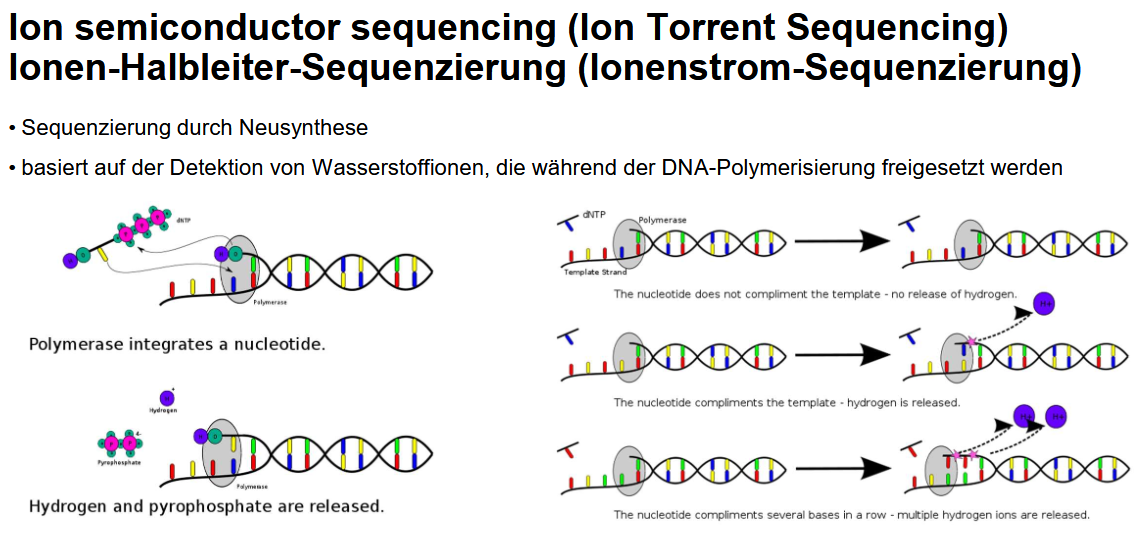
\includegraphics[width=1\linewidth]{images/ION1.PNG}
    \caption{Prinzip der Freisetzung von Wasserstoff bei der Ionen-Halbleiter-Sequenzierung}
    \label{fig:enter-label}
\end{figure}
\begin{figure}[H]
    \centering
    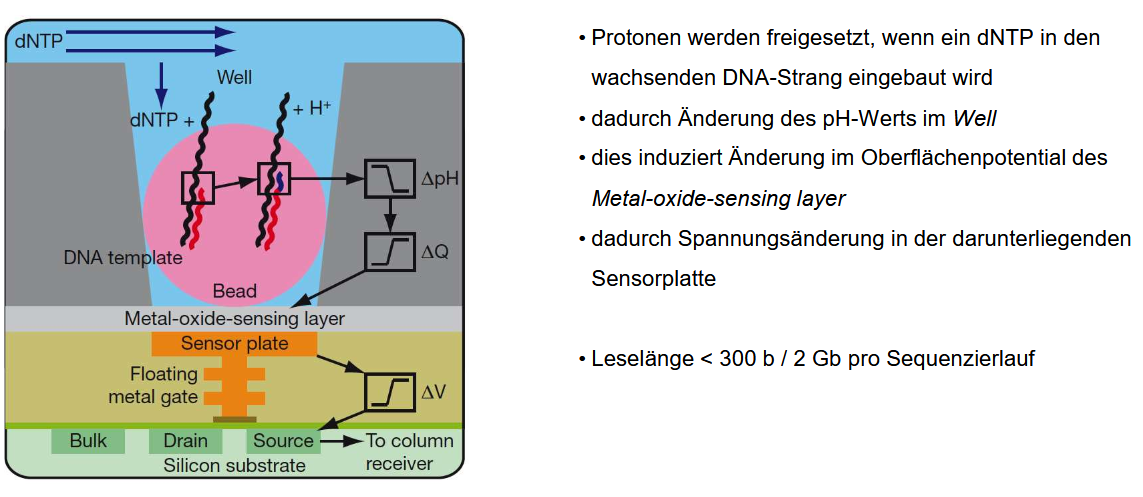
\includegraphics[width=1\linewidth]{images/Ion2.PNG}
    \caption{Aufbau und prozessierung der Wasserstoff freisetzungen}
    \label{fig:enter-label}
\end{figure}

\section{3rd Generation Sequenzierung}\index{Sequenzierung!3rd Generation}
\subsection{PACBIO RS} \index{Sequenzierung!PACBIO RS}
\begin{figure}[H]
    \centering
    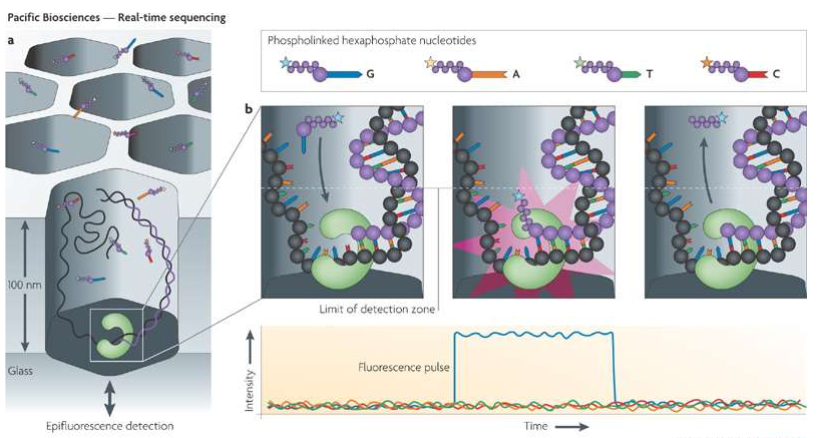
\includegraphics[width=0.9\linewidth]{images/PacBio.PNG}
    \caption{Funktion der DNA Polymerase und markierten Nukleotiden}
    \label{fig:enter-label}
\end{figure}

\begin{mechanism}[title=Was ist PACBIO-SMRT-Sequencing?]
Eine Single-Molecule Sequencing-Methode, die Sequenzierung in Echtzeit und ohne vorherige Amplifikation ermöglicht.  \\
Während die DNA-Polymerase die DNA repliziert, werden fluoreszenzmarkierte Nukleotide eingebaut. Die Fluoreszenzfarbstoffe befinden sich an den Phosphatgruppen der Nukleotide. Sobald ein Nukleotid eingebaut ist, wird der Farbstoff abgespalten und erzeugt ein Fluoreszenzsignal.
\end{mechanism}

\subsection{Nanopore}\index{Sequenzierung!Nanopore}
\begin{figure}[H]
    \centering
    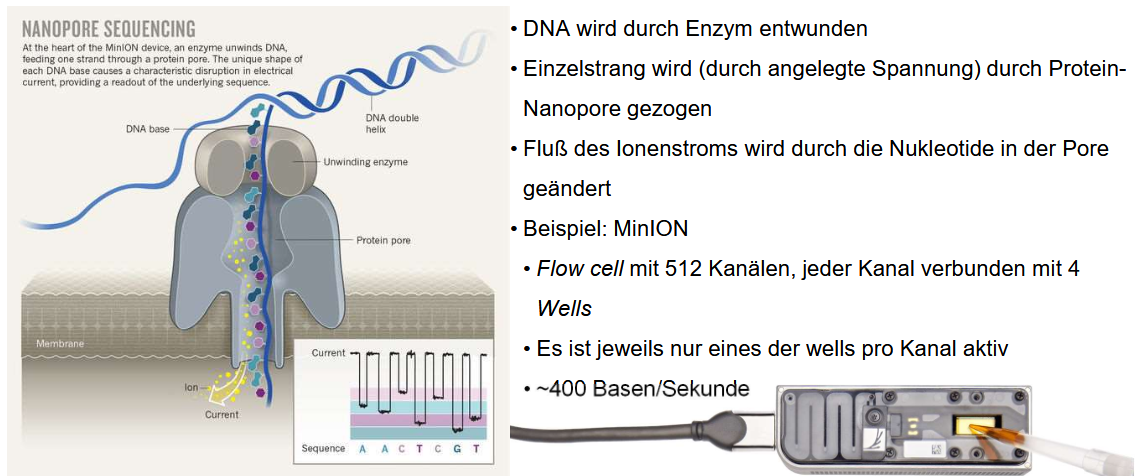
\includegraphics[width=1.2\linewidth]{images/Nanopore.PNG}
    \caption{Nanopore Kanal mit Erläuterung des Aufbaus und Ablauf}
    \label{fig:enter-label}
\end{figure}

\begin{mechanism}[title=Unterschied Illumina vs. Nanopore]
Der signifikante Unterschied liegt hierbei darin, dass Illumina eine synthetisch
basierte ”short read” Sequenzierung ist. Characteristisch für solche sind ihre
Cluster an vielen kurzen Sequenzen.
Nanopore hingegen ist eine ”long read” Sequenzierung. Dies wird ermöglicht
durch elektronische Spannungsunterschiede bei Nukleotiden in der Nanopore.
\end{mechanism}

\begin{mechanism}[title=Was sind die Nachteile von Oxford Nanopore?]
Hohe Fehlerrate und Anschaffungskosten sehr hoch
\end{mechanism}
\begin{mechanism}[title=Was sind die Vorteile langer Reads?]
Direktes Lesen von epigenetischen Modifikationen und direkte Sequenzierung einzelner DNA-Moleküle
\end{mechanism}

\begin{mechanism}[title=Durch einen Sequenzierfehler wurde eine zusätzliche Base in die Sequenz eingebaut. Welche späteren Folgen kann dies haben?]
Durch die Insertion wurde das Leseraster der Basentrippletts verändert. Somit kann es zu missinterpretationen der Proteinsequenzen und oder zu falschen bzw. keinen Ergebnissen in dem Datenbank abgleich führen.
\end{mechanism}
